\documentclass[10pt,a4paper]{article}
\usepackage[utf8]{inputenc}
\usepackage[english]{babel}
\usepackage{graphicx}
\usepackage{url}
\author{Ken LE PRADO}
\title{Modbus Testbed}
\begin{document}

\section{Introduction}
	
	Modbus\footnote{\url{http://www.modbus.org}} is a network protocol commonly used for Industrial Systems.
	Learning and testing on this protocol is essential on a physical testbed.
	A testbed based on Lego Mindstorms is a cheap and flexible solution.
	
	This document describes the realization of a Lego Mindstorms EV3 test bed for Modbus.

\section{General description}
	The testbed is composed of :
	\begin{itemize}
	    \item a Management Terminal Unit (MTU),
	    \item multiples Remote Terminal Unit (RTU),
	    \item a network for communications between MTU and RTU with Modbus.
	\end{itemize}

	The protocol used to communicate between RTU and its sensors (I2C) or actuators (PWM) is imposed by the Lego Mindostorms EV3 device.
		
	The model used is a lift bridge preceded by one or multiple tolls. These elements (RTU) does not communicates together. Only the control center (MTU) read the RTU states and modify their registers. The Human-Machine Interface (IHM) display status and permit to activate the RTU.
	
	
    Technology deployed :    
    \begin{description}
        \item[Lejos\footnote{http://www.lejos.org}] This open-source framework permit a Java development for Lego Mindstorms. Lejos comes with a Linux distribution to install on the Mindstorms EV3, and a plugins for Eclipse IDE.
        \item[Jamod\footnote{http://jamod.sourceforge.net}] Java library to manage the Modbus communications. This library has been modfy in order to implement new Modbus function codes.
    \end{description}
		
	\begin{center}
	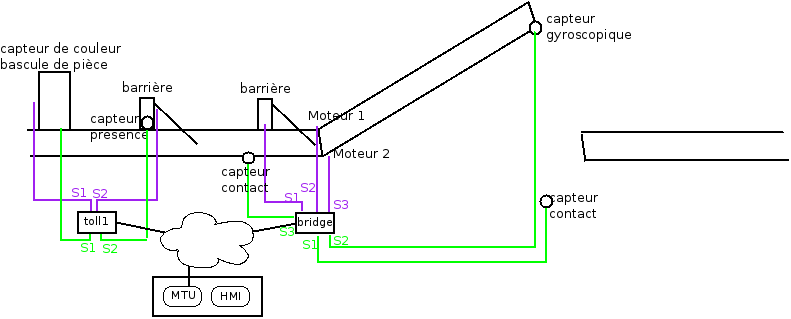
\includegraphics[height=5cm]{rsrc/schema_peage-pont.png}
	\end{center}

\section{RTU}
	Each RTU inherit a Device class which defines a RTU. A toll or a bridge extends the class Device\footnote{the full Javadoc documentation is available}, which permit to define easily a new component.
	
	\begin{center}
	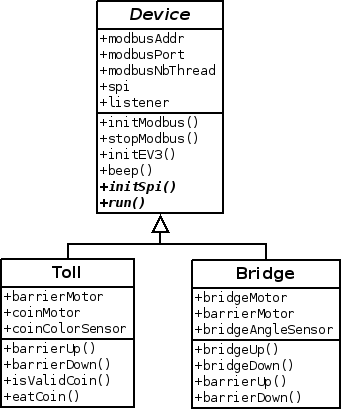
\includegraphics[height=6cm]{rsrc/Device_class.png}
	\end{center}
		
	\subsection{Toll}
		
		A toll system is simple and may be reproduced on the testbed. A simulated implementation has been implemented (TollSim class).
		
		\begin{center}
		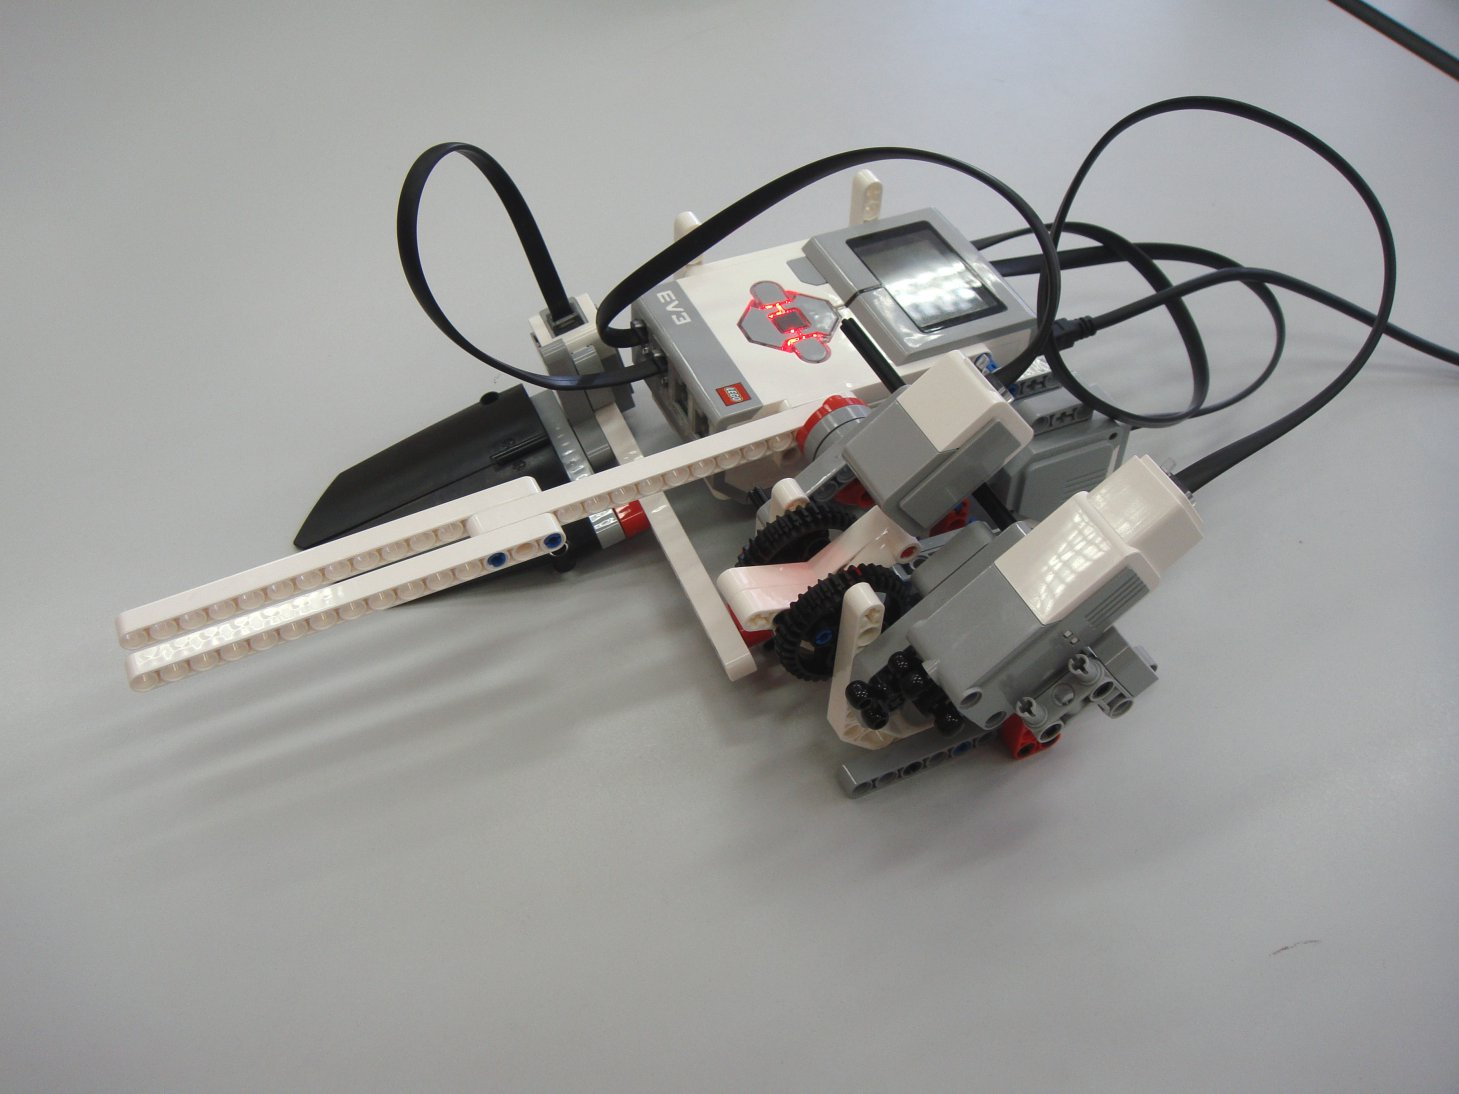
\includegraphics[height=4cm]{rsrc/Toll_01.jpg}
		\end{center}
		
	    \subsubsection{Register definition}
		
			\begin{tabular}{|c|c|l|l|}
			\hline 
			\textbf{Type} & \textbf{Ref} & \textbf{Name} & \textbf{Description} \\ 
			\hline 
			Input register & 0 & UNIT\_ID & Unit Identifier\\ 
			\hline 
			Input register & 1 & COIN\_COLOR & Coin color sensor value\\ 
			\hline 
			Input register & 2 & CAR\_TOUCH & Car hit sensor value\\ 
			\hline 
			Input register & 3 & KEY\_PRESS & EV3 button hit sensor value\\ 
			\hline 
			Register & 0 & NB\_CARS & Viewed cars\\ 
			\hline 
			Register & 1 & NB\_COINS & Eated coins\\ 
			\hline 
			Coil & 0 & ACTIVE & Toll activation status \\ 
			\hline 
			Coil & 1 & FREE & Toll payment status (free/paying) \\ 
			\hline 
			Discrete Input & 0 & BARRIER & Barrier position (true = opened) \\ 
			\hline 
			\end{tabular} 
		
	\subsection{Lift bridge}
	A lift bridge is an interesting element which has to be safety for the cars. A visible security problem may have direct consequences.
	
	\begin{center}
	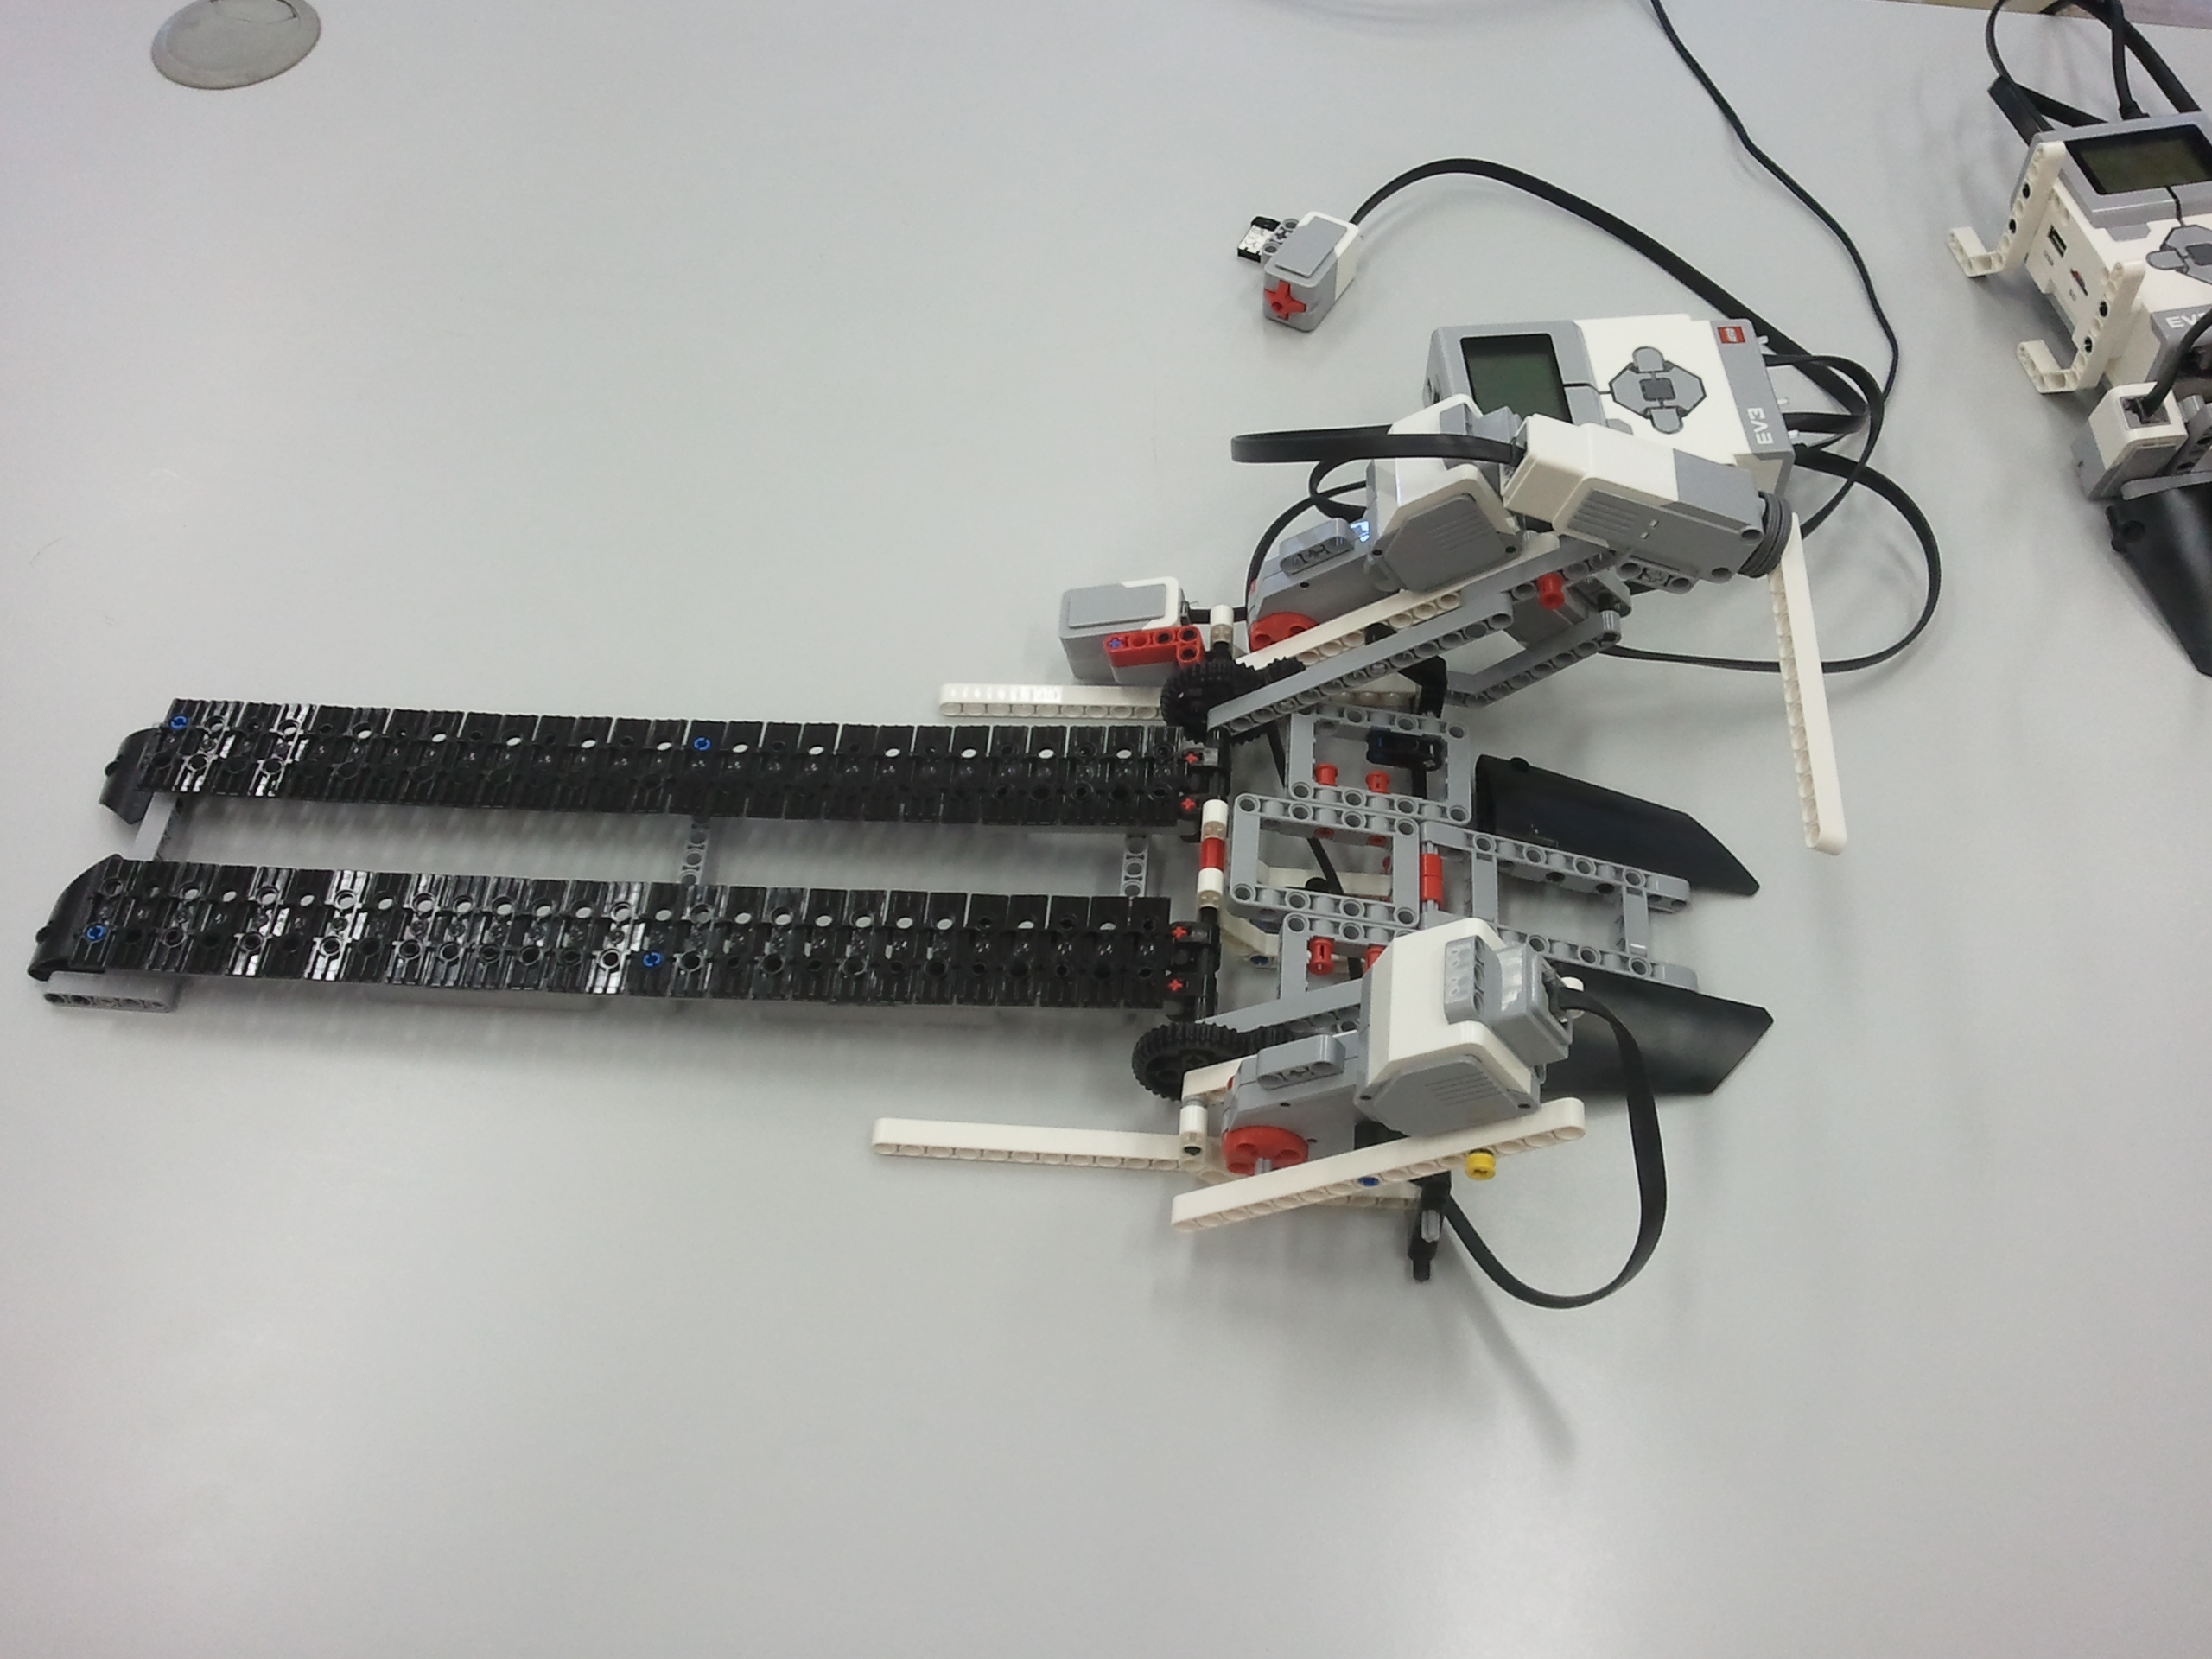
\includegraphics[height=4cm]{rsrc/Bridge_02.jpg}
	\end{center}
	
	    \subsubsection{Register definition}
	
		\begin{tabular}{|c|c|l|l|}
		\hline 
		\textbf{Type} & \textbf{Ref} & \textbf{Nom} & \textbf{Description} \\ 
		\hline 
		Input register & 0 & UNIT\_ID & Unit Identifier\\ 
		\hline 
		Input register & 1 & SENSOR\_BUTTON & EV3 button sensor value\\ 
		\hline 
		Input register & 2 & SENSOR\_GYRO & Gyroscopic sensor value\\ 
		\hline 
		Input register & 3 & SENSOR\_PASSAGE & Car hit sensor value\\ 
		\hline 
		Input register & 4 & SENSOR\_BOAT & Boat hit sensor value\\ 
		\hline 
		Input register & 5 & SENSOR\_MOVE & Bridge movement (0 : stopped, 1 : up, 2 : down) \\ 
		\hline 
		Input register & 6 & SENSOR\_ANGLE & Angle value computed by motors\\ 
		\hline 
		Register & 0 & NB\_CARS & Cars viewed\\ 
		\hline 
		Coil & 0 & ACTIVE & Bridge activated\\ 
		\hline 
		Coil & 1 & BRIDGE\_MOVE & Bridge movement requested\\ 
		\hline 
		Coil & 2 & BRIDGE\_RAISE & Way of the bridge movement requested\\
		\hline 
		Coil & 3 & BARRIER\_OPENED & Barrier position requested\\ 
		\hline 
		Discrete Input & 0 & BARRIER & Barrier position (true = opened) \\ 
		\hline 
		Discrete Input & 1 & WAITING\_BOAT & Boat waiting status\\ 
		\hline 
		\end{tabular} 
		
\section{Control Center}
    The control center integrates the MTU and HMI functions. It is the Master in the Modbus communications.
    
	\begin{center}
	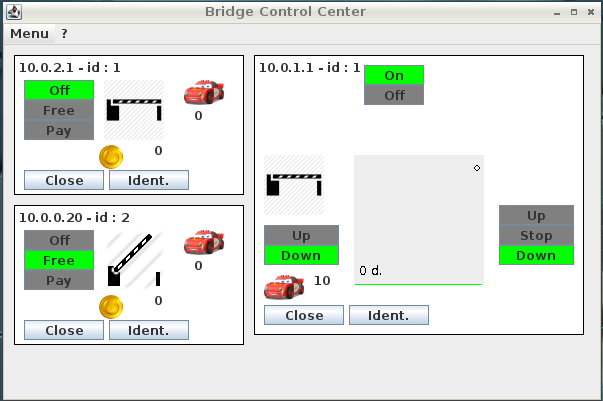
\includegraphics[height=4cm]{rsrc/CC_screenshot.png}
	\end{center}


\section{Testbed consideration}

    This testbed implements Modbus for communications and permits to test the security.
    
\end{document}